\chapter{「程序」是怎样炼成的}
\label{cha:program-and-arch}

\begin{intro}
  近些年,大街小巷上,「编程辅导」的广告层出不穷;中小学校里,程序设计的知识走进了课堂。在这股浪潮之下,你是否想过这样一个看似简单却难以言说的问题——「程序」是什么?它们又是如何运行的?看完这一章,你或许可以找到这些问题的答案:

  \begin{itemize}
    \item 什么是「程序」?「编程」是要做什么?
    \item 什么是 Python、C 语言、C++、Java……
    \item 各种各样的程序,是如何在电脑的硬件上运行的?
    \item 什么是「32 位」「64 位」?什么是「x86」,什么是「ARM」?
  \end{itemize}

  在开始之前,我们还需强调:《你缺计课》不是一本编程书。我们不会深入介绍任何编程语言,更不会教你代码怎么写。相反,我们将聚焦宏观和整体,向你展示「『程序』是怎样炼成的」。
\end{intro}

早在《你缺计课》的第一章\chapref{cha:computer-and-its-components}我们就介绍过,电脑是由硬件和软件组成的有机整体。事实上,我们身边的平板电脑、手机、智能手表……一切智能设备,都由硬件和软件组成。这里面,硬件对应着电路、芯片以及各种外部设备,而软件就对应着各种各样的\regcolor{计算机程序},简称\regcolor{程序}。

我们在电脑、手机上运行的各种软件(app),它们的本质是一个个程序。而 Windows、iOS、安卓这些操作系统,它们亦是一类特殊的程序。编写程序的过程就是「编程」,这是今天许多人的工作。那么,这各种各样的程序是如何被设计出来的呢?千变万化的程序,又是怎么在看似呆板的硬件上运行的呢?本章,让我们揭开「程序」这个熟悉却陌生之物的面纱,了解它背后的秘密。

\section{程序?菜谱!}

\subsection{大事化小的程序思维}

「程序思维」,听起来是个很抽象的词。的确,不如先把它放到一边,让我们来看看生活中常见的「做菜」情景。番茄炒蛋是一道经典的家常菜,我们可以将烹饪它的过程归纳为这样的 5 个步骤:

\begin{itemize}
  \item 备菜:打蛋、洗净番茄切块;
  \item 单炒鸡蛋:将鸡蛋炒至基本成型但保持嫩滑的状态,待用;
  \item 单炒番茄:将番茄炒至变软,略开始出汁的状态;
  \item 合炒、调味:将之前炒好的鸡蛋倒入,翻炒均匀,加入调味料;
  \item 出锅。
\end{itemize}

\begin{figure}[htb!]
  \centering
  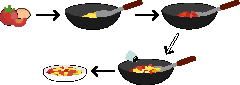
\includegraphics[width=.65\textwidth]{assets/surpass/Tomato_egg.pdf}
  \caption{如何做番茄炒蛋}
  \label{fig:Tomato_egg}
\end{figure}

对会做菜的读者来说,这份步骤表已经足以帮助你做出一盘番茄炒蛋了。然而,如果你是一位从未下过厨房的读者,它就略显笼统了。在这种情况下,我们不妨「大事化小」,先约定一系列最简单、最基本的操作,如「切」「洗」「翻炒」等。这些操作单一而机械,可以在很短的时间内掌握。借助它们,我们就能得到一份这样的菜谱:

\begin{multicols}{2}
  \begin{itemize}
    \item 备菜:
      \begin{itemize}
        \item \textbf{洗} \underline{番茄} 3 个 → 得到「洗净的番茄」;
        \item \textbf{切} \underline{洗净的番茄} → 得到「番茄块」;
        \item \textbf{打} \underline{鸡蛋} 4 个 → 得到「鸡蛋液」;
      \end{itemize}
    \item 单炒鸡蛋:
      \begin{itemize}
        \item \textbf{点火};
        \item \textbf{向锅中加入} \underline{油} 20 mL;
        \item \textbf{等待} 20 秒;
        \item \textbf{向锅中加入} \underline{鸡蛋液};
        \item \textbf{翻炒} 40 秒;
        \item \textbf{熄火};
        \item \textbf{从锅中取出} \underline{炒好的鸡蛋} → 得到「炒好的鸡蛋」;
      \end{itemize}
    \item 单炒番茄:
      \begin{itemize}
        \item \textbf{点火};
        \item \textbf{向锅中加入} \underline{油} 10 mL;
        \item \textbf{等待} 10 秒;
        \item \textbf{向锅中加入} \underline{番茄块};
        \item \textbf{翻炒} 1 分 20 秒;
      \end{itemize}
    \item 合炒、调味:
      \begin{itemize}
        \item \textbf{向锅中加入} \underline{炒好的鸡蛋};
        \item \textbf{翻炒} 1 分钟;
        \item \textbf{向锅中加入} \underline{盐} 2 g;
        \item \textbf{翻炒} 20 秒;
        \item \textbf{熄火};
      \end{itemize}
    \item 出锅:
      \begin{itemize}
        \item \textbf{从锅中取出} \underline{番茄炒蛋} → 得到一盘「番茄炒蛋」。
      \end{itemize}
  \end{itemize}
\end{multicols}

这份详细的菜谱中,只包含几类基本操作,而且每一步操作都被精确、定量地描述。理论上,借助它,即使是完全没有烹饪经验的人,也可以在简单培训后完成任务。

「程序思维」的含义,就隐含在这菜谱中——将大事化为小事,通过组合利用少量、基础的操作,完成一项庞大、复杂的任务的思维。在计算机的世界里,系统只提供少量最基本的操作,如简单的算术运算,以及「读取文件」「显示内容」等交互动作。程序就像一份菜谱:\regcolor{通过组合运用基本操作,实现各种各样的功能};而编程的过程,就是我们利用程序思维来编写如上「菜谱」的过程。所以,从这个角度而言,这份菜谱,本质上是一份「程序」的「\regcolor{源代码}」,只不过处理它的设备并非计算机,而是我们人类。

\subsection{顺序、分支与循环结构}

之前的菜谱「程序」中,所有操作都是完全固定的——从食材的量到翻炒的时间,都以具体的数字约束起来。然而,在现实生活中,起锅烧油所需要的时间可能与油的品质、气温、油量的多少等因素有关,而翻炒的时间也和食材的新鲜程度、切片时的厚度等挂钩。无疑,这个程序无法适应环境的任何改变。为此,我们再引入一种这样的操作:

\begin{itemize}
  \item \textbf{如果} \underline{番茄块} 还没有变软:
    \begin{itemize}
      \item 再 \textbf{翻炒} 10 秒;
    \end{itemize}
  \item \textbf{否则}:
    \begin{itemize}
      \item 什么也不做。
    \end{itemize}
\end{itemize}

相比于原来「做完一件事,就顺着做下一件事」的一刀流,在引入这种「如果」操作后,我们的程序长出了分支。在番茄比较生、气温比较低,或者水放多了的情况下,程序会进入「再翻炒 10 秒」这一支;而当番茄质地偏软、天气炎热,又或者灶台火力较猛时,程序就会选择什么也不做,然后离开分支继续向后运行。我们把原来的程序结构称为「顺序结构」,而\regcolor{这种引入「如果」的结构称为「分支结构」}。

我们可以将这种结构用「流程图」的方式展现出来,如下图左侧所示。

\begin{figure}[htb!]
  \centering
  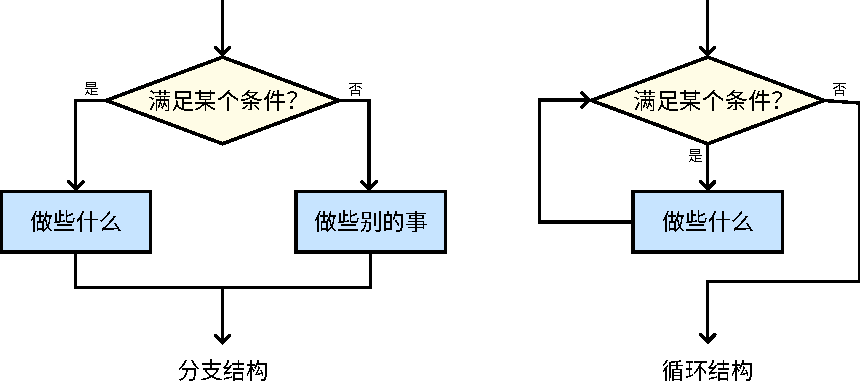
\includegraphics[width=.8\textwidth]{assets/surpass/Branch_and_loop.pdf}
  \caption{分支与循环结构}
  \label{fig:Branch_and_loop}
\end{figure}

可是,分支结构只能实现「二选一」,就算多个分支套起来也只能实现「三选一」「四选一」……套太多分支会显得过于复杂,同时程序能走出的道路仍是有限的。上面的例子让我们得以给还不够熟的番茄多炒 10 秒,可是如果 10 秒还不够呢?相反,如果火力过大,原本设定的 1 分多钟翻炒下来,番茄可能已经成炭了。分支结构在这样的情况下,「心有余而力不足」。为了解决这个问题,我们需要一种新的操作:

\begin{itemize}
  \item \textbf{当} \underline{番茄块} 还没有变软 时:
    \begin{itemize}
      \item 再 \textbf{翻炒} 10 秒。
    \end{itemize}
\end{itemize}

乍一看,这个操作的形式和刚刚提到的「如果」挺相似,但是含义完全不同。这个操作是说,\regcolor{只要番茄块还没有变软,就一直重复}执行「翻炒 10 秒」这一步。只有某时刻,「番茄块还没有变软」的条件不满足了,才能离开这个轮回。\regcolor{这种构称为「循环结构」,而循环内执行的操作就是这个循环的「循环体」}。顾名思义,循环结构的作用就是在一定的条件下,不断重复地做同一件事,直到这个条件不再成立。相较之下,分支结构也需要检查某个条件,但分支的操作只会执行一次。循环结构的流程图如\autoref{fig:Branch_and_loop} 右侧所示。

\begin{note}
  分支结构和循环结构有明显的不同,但是,只要再引入一种操作,就能让分支结构变为循环结构。这个操作就是「跳转」,其目标是某个步骤。例如,下面的程序没有使用循环结构的「当」操作,却实现了和上面的程序完全一样的效果。
  \begin{enumerate}
    \item \textbf{如果} \underline{番茄块} 已经变软:
      \begin{itemize}
        \item \textbf{跳转到} 第 4 步;
      \end{itemize}
    \item \textbf{翻炒} 10 秒;
    \item \textbf{跳转到} 第 1 步;
    \item (继续后面的步骤。)
  \end{enumerate}

  不妨借助流程图分析为什么这种转换得以成立。
\end{note}

那么,我们可以将原本固定的 4 分钟翻炒直接替换为上面的循环,这样,我们的菜谱程序一开始就可以根据番茄是否变软来控制翻炒的时间,实现了「具体问题具体分析」。进一步,我们还可以把循环体中的「10 秒」缩得更短,这样程序控制的精度就更高。

\regcolor{顺序、分支和循环结构是程序的三种基本控制结构}——事实上,只需要这三种结构,就能将世间一切复杂之事,用程序思维分解为基础操作的组合。你不妨现在思考一下身边各种各样的事:小到日常生活中的鸡毛蒜皮,大到社会运行的底层原理,一切都可以归约成这三种结构组合之下的基本操作。这就是程序思维的力量,也是今天的数字世界能够诞生的重要基石。

\subsection{编程语言}

在上一小节中,我们设计了一个菜谱「程序」,并用中文写出了它的「源代码」:对于这个程序的每一步,我们都使用完整的中文句子来描述它的含义。然而,世界上的语言千千万,我们大可以使用不同的语言来描述它——只要保持含义不变,那么整个程序的本质和功能就没有改变。例如,我们可以用英语来描述「炒鸡蛋」这一段,除了得到的源代码长得不一样之外,它们在功能上是一致的:

\begin{itemize}
  \item Scramble Eggs:
    \begin{itemize}
      \item \textbf{Light the stove};
      \item \textbf{Add} 20 mL of \underline{oil} \textbf{to the wok};
      \item \textbf{Wait} for 20 seconds;
      \item \textbf{Add} \underline{egg wash} \textbf{to the wok};
      \item \textbf{Scramble} for 40 seconds;
      \item \textbf{Turn off the stove};
      \item \textbf{Set} \underline{scrambled eggs} \textbf{aside}.
    \end{itemize}
\end{itemize}

诸如中文、英语、法语这样的自然语言,是我们人与人之间沟通的「桥梁」,而借助这样的桥梁,我们才得以用菜谱来指导他人完成烹饪。在真正的程序世界中,人们亦设计了无数种不同的「编程语言」。我们同样可以利用不同的编程语言,实现相同的功能。例如,为了计算
\[ \sum_{i=1}^{100} i^2=1^2+2^2+\cdots+99^2+100^2\text{,} \]
我们可以用程序思维,设计出下面的计算流程:

\begin{itemize}
  \item \textbf{令} \underline{sum} 为 0;
  \item \textbf{令} \underline{index} 为 1;
  \item \textbf{当} \underline{index} 小于或等于 100 时:
    \begin{itemize}
      \item \textbf{给} \underline{sum} \textbf{加上} \underline{index} 的平方;
      \item \textbf{给} \underline{index} \textbf{加上} 1;
    \end{itemize}
  \item \underline{sum} 就是最终的答案。
\end{itemize}

接着,我们使用几门编程语言「C 语言」「C++」「Java」「Python」「Rust」和「文言\footnote{「文言」(wenyan-lang)还真是一门编程语言哦,你可以在它的官方网站 \url{https://wy-lang.org/} 查看更多信息。}」,来将这个思路写成代码:

\begin{MissingVerbatim}[c]
#include <stdio.h>
int main() {
    int sum = 0;
    for (int i = 1; i <= 100; ++i) {
        sum += i * i;
    }
    printf("答案是 %d", sum);
    return 0;
}
\end{MissingVerbatim}

\begin{MissingVerbatim}[cpp]
#include <iostream>
int main() {
    int sum = 0;
    for (int i = 1; i <= 100; ++i) {
        sum += i * i;
    }
    std::cout << "答案是 " << sum << std::endl;
    return 0;
}
\end{MissingVerbatim}

\begin{MissingVerbatim}[java]
public class SumOfSquares {
    public static void main(String[] args) {
        int sum = 0;
        for (int i = 1; i <= 100; i++) {
            sum += i * i;
        }
        System.out.println("答案是 " + sum);
    }
}
\end{MissingVerbatim}

\begin{MissingVerbatim}[python]
print("答案是", sum(i**2 for i in range(1, 101)))
\end{MissingVerbatim}

\begin{MissingVerbatim}[rust]
fn main() {
    let sum = (1..=100).map(|i| i * i).sum::<i32>();
    println!("答案是 {}", sum);
}
\end{MissingVerbatim}

\begin{MissingVerbatim}
吾有二數。曰一。曰零。名之曰「計」。曰「和」。
為是百遍。
  乘「計」以「計」。加其以「和」。昔之「和」者。今其是矣。
  加「計」以一。昔之「計」者。今其是矣。
云云。

夫「「答曰」」。夫「和」。書之。
\end{MissingVerbatim}

纵览这几份使用不同编程语言写成的源代码,会发现它们风格各有不同:C 语言与 C++ 长得几乎一样,而二者和 Java 亦有几分相似。再仔细一看,会发现它们其实与我们用人类语言描述思路的结构类似。Python 和 Rust 则有更短的代码长度,Python 甚至在一行内就解决了问题,但是代码就不那么直观了。而至于那颇有我国古代数学著作风格的「文言」,则较 C/C++ 更甚,更加直观地刻画了我们的思路。这提醒我们:不同的编程语言有自己的「性格」,亦有自己的适用范围。

除了「文言」之外,上面提到的几门编程语言在当下都比较常用,这里简要介绍一下。

\begin{itemize}
  \item C 语言是 C++ 的「祖宗」,具体来说,C++ 去掉了 C 中少许不妙的特性,但增加了许多更妙的功能,因此人们常用「C/C++」这样的名字来并称它们。它们是相当基础的编程语言,下限较低、上限很高,因此用途非常广泛。\regcolor{大多数操作系统,包括我们正在使用的 Windows,底层都使用 C/C++ 开发。}同时,大量的电脑软件、游戏引擎、乃至《你缺计课》的服务端软件\footnote{我们使用 NGINX。它会在你访问我们的网站时,把网页的内容发送给你。}都是使用 C/C++ 编写的。
  \item Java 相比与 C++,具有更清晰的语法,编写难度较低,既容易学习又功能丰富,同时它还是曾经开发安卓 app 的首选(或者说是唯一)语言。至今,\regcolor{大量的安卓 app 中仍有许多 Java 代码}。此外,很多服务端软件、电脑游戏《我的世界》都使用 Java 开发。
  \item Python 是一门极为灵活的语言(诨名「胶水语言」)——同样的任务,它可以用多种方式实现,能写出非常简洁的代码,并同时保持一定的可读性。Python 还是一门非常开放的语言:它拥有一个庞大的社区,其中\regcolor{有许多别人写好的「库」供我们直接使用,这些库让 Python 几乎无所不能}。不过,Python 的运行速度很慢。这决定了 \regcolor{Python 主要被用在数据分析、科学研究、人工智能等领域},而不是用来编写「真正干活的」软件。也基于类似的原因,Python 成了现在「编程入门」的标配。
  \item Rust 是一门新兴的编程语言,诞生至今不过十余年。它吸收了来自多种不同编程语言的优秀设计,并以「安全」作为一大特色——这能在一定程度上减少程序中漏洞的产生。目前,Rust 正在快速发展,并已经在产业界有些应用——Linux 操作系统就开始使用 Rust 编写一部分代码。
\end{itemize}

然而,世间有数不尽的编程语言,每年都会有无数新的语言诞生,各自标榜自己具有这样那样的优势,也有许多曾经雄心勃勃的语言变得无人问津、逐渐消亡。但总之,\regcolor{学习一门编程语言并不是难事——相反,最难的事情终究是「如何运用程序思维将问题分解」}。只要拥有这样的思维,无论使用什么语言,你会发现它们的思想是共通的。下面,我们将简要地介绍「算法」,来更深刻地体会思维的重要性。

\subsection{用好算法,事半功倍}

在中小学学习数学的过程中,老师都喜欢强调一个概念——「一题多解」。通常,一道题不止有一种解法;但是这不同的解法之间,往往在复杂度和用时方面有差距。例如,解决立体几何问题,就有建立坐标系的「解析法」和利用几何关系的「直接计算法」。在程序设计的世界里,实现相同的功能,亦有着不同的方式。我们把\regcolor{一套定义好的,可以由计算机按指示执行的步骤称为一种「算法」(algorithm)}。显然,解决同一个问题往往可以运用许多种不同的算法,而算法之间就有了优劣之分。

假设现在我们要设计一个程序来炒出 100 盘番茄炒蛋。最简单的想法,便是重复执行 100 遍此前的的菜谱程序。这样做的确可行,然而,由于做每一盘都需要重复多次起锅烧油的过程,若再考虑实际场景,在「炒鸡蛋」和「炒番茄」两步之间来回切换亦十分消耗时间,这样做的效率无疑相当低下。为了缓解这个情况,我们可以选择最「大」化利用我们的锅:假如我们的锅一次最多能炒 10 盘菜的量,我们就可以一次炒 10 倍的鸡蛋,再一次性炒出 10 盘菜来。这样,重复操作的次数就从原来的 100 次下降为 10 次——换算成时间,这大大减少了开销。

\begin{note}
  根据前文菜谱中给出的时间数值,计算采用这种方式能节省的时间。
\end{note}

这个例子虽然简单,但是它向我们强调了好算法的重要性:同样的问题,选择好的算法能节省更多的时间;在相同的时间内,选择好的算法又能解决更多的问题。我们再来分析一个问题:如果要计算 1 到 100 的阶乘\footnote{$n! = 1\times2\times3\times\cdots\times(n-1)\times n$}和,也即
\begin{align*}
  \sum_{i=1}^{100}i!&=1!+2!+\cdots+99!+100! \\
  &=1+1\times 2+1\times 2\times 3+\cdots+1\times 2\times 3\times\cdots\times 100\text{,}
\end{align*}

最简单的想法是逐个计算每一项阶乘的值:$1!$、$2!$、$3!$……一直到 $99!$ 和 $100!$,然后把它们相加。但用这种方式,我们看看要做多少运算:

\begin{itemize}
  \item 乘法:$1!$ 无需乘法,$2!$ 需要 1 次,$3!$ 需要 2 次……$100!$ 需要 99 次。一共乘了 4950 次;
  \item 加法:100 个数相加,一共 99 次。
\end{itemize}

显然,大部分时间花在了那几千次乘法运算上。但阶乘运算有点特殊,$2! = 2\times 1!$,$3! = 3\times 2!$……$100! = 100\times 99!$,后一个阶乘只需在前一个阶乘的结果上多乘一个数得到。这样一来,一个新的思路就呼之欲出了,我们可以把计算流程变成:

\begin{itemize}
  \item 先计算 $1! = 1$;
  \item 再计算 $2! = 2 \times 1! = 2$;
  \item 再计算 $3! = 3 \times 2! = 6$;
  \item 再计算 $4! = 4 \times 3! = 24$;
  \item ……
  \item 再计算 $100! = 100 \times 99! = 93326215 \cdots 0000$。
\end{itemize}

最后将这 100 个结果相加即可。新的流程中,每一步都基于上一步的结果计算,只需要一次乘法,因此总共进行了 99 次乘法和 99 次加法。与之前相比,我们将运算量减少到了原来的 4\%:如果原来的计算需要 100 毫秒,那么现在的计算就只需要 4 毫秒。对于许多问题,一个好的算法能让我们不止事半功倍。

\begin{note}
  如果你已经学过编程,或打算学习编程,不妨在习得一门编程语言后按照不同的算法编写计算上述问题的不同程序,感受好算法带来的性能提升。(计算机运行得很快,你可能需要进一步增大问题的规模,并精确计时。)
\end{note}

在计算机理论领域,人们针对排序问题、搜索问题、图论问题等大量的经典问题研究出了许多优秀的算法。而这些经典的优秀算法,早已在各大编程语言中实现成可以直接使用的「方法」,让人们在编程时可以直接「站在巨人的肩膀上」。

\section{0 与 1 的圆舞曲}

至此,我们已经明白,通过各种各样的编程语言,借助程序思维,人们得以将需要完成的工作用程序呈现;而通过研究算法,程序的效率又能得到极大提升,从而更有效地解决问题。然而,我们所认识的「程序」,与呆板的芯片、导线、电路所构成的计算机硬件之间,依然还隔着一道天堑。程序奏响的思维之韵,是如何化为 0 与 1 的圆舞曲的?下面,就由我们为你一一道来。

\subsection{程序、指令、机器代码}

在\chapref{cha:characters-and-encodings}一章中我们提到,计算机中的一切信息都由电路承载:每条信息都是由若干位 0 和 1 这样的二进制数字所组成,反映在电路上,就是「有电」「无电」之间的排列组合。为了在硬件上运行程序,我们自然就先得寻找「程序」在硬件上的表达方式,或者说,将程序由源代码转换为 0 和 1 的序列的方式。

上一节,我们构想了一个番茄炒蛋菜谱「程序」,不过那时程序预计的「硬件」就是我们人类。现在,我们想做一台炒菜机器「你缺饭课一号」,让它代替人类来执行这份程序。然而,「你缺饭课一号」并不能看懂中文、英文这样的人类语言,因此不能直接看懂那份「源代码」。作为炒菜机器,它能做的,就是不断读取某处并排的 8 根导线上传来的信号(它们代表一个 8 位二进制数),然后根据这组信号的值,执行一个简单的动作。那么,我们可以给「你缺饭课一号」赋予这样的设计:

\begin{figure}[htb!]
  \centering
  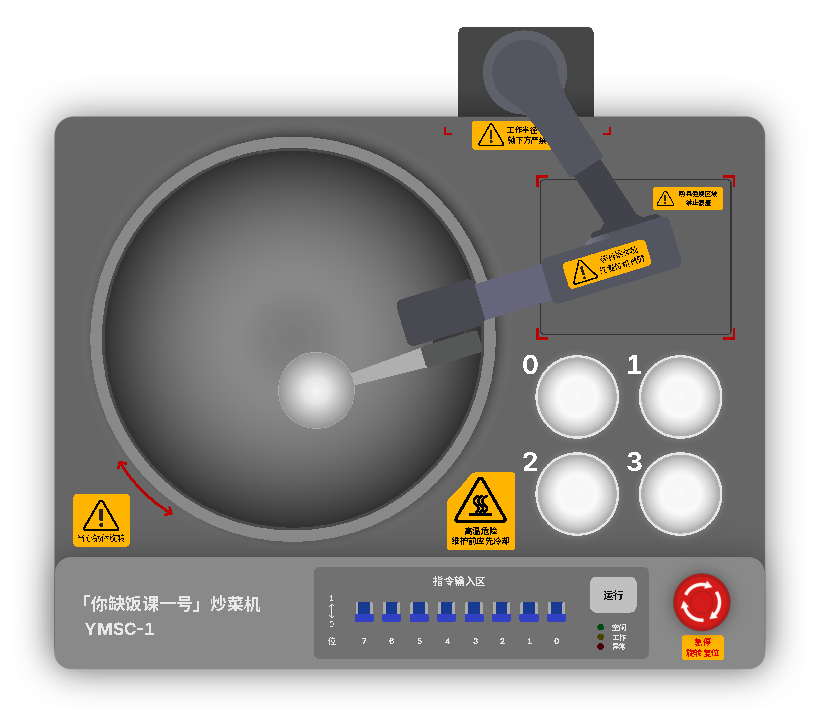
\includegraphics[width=.65\textwidth]{assets/surpass/YMSC-1.pdf}
  \caption{隆重推出「你缺饭课一号」!}
  \label{fig:YMSC-1}
\end{figure}

\begin{itemize}
  \item 机器一共有 4 个碗,依次编号 0、1、2、3,可以在烹饪过程中装食材、食物。
  \item 机器不断读取传来的 8 位信号,并按照下面的规则选择动作:
    \begin{longtblr}[
      caption   = {「你缺饭课一号」功能表},
      label     = {tab:YMSC-1-func},
    ]{
      colspec   = XX[5],
      rowhead   = 1,
      row{1}    = {halign=c, fg = white, bg = missing, font = \bfseries},
      row{even} = {MissingSkyBlue},
      column{1} = {halign=c},
      cells     = {valign=m},
    }
      \toprule
      信号 & 功能 \\
      \midrule
      \MissingTT{0001xxyy} & {洗一份食材。\MissingTT{xx} 决定食材的种类:\MissingTT{00} 代表番茄、\MissingTT{01} 代表青椒……\\\MissingTT{yy} 表示洗完之后的食材加到哪个碗里,一共有 \MissingTT{00} 至 \MissingTT{11} 四个碗可以使用。\\例如,信号 \MissingTT{00010000} 能控制机器洗一份番茄放到第 0 号碗里。} \\
      \MissingTT{001000yy} & 打鸡蛋。\MissingTT{yy} 决定打好的蛋放在哪个碗里。 \\
      \MissingTT{001100yy} & 切菜。将 \MissingTT{yy} 号碗中的食材全部切块。 \\
      \MissingTT{01000xxx} & 给灶台点火,并向锅中加入 $10\times\overline{\text{xxx}}_{\mathrm{B}}$ mL 的油。例如,\MissingTT{01000100} 对应的 \MissingTT{xxx} 是 \MissingTT{100},也就是点火后加入 $10\times4=40$ mL 的油。 \\
      \MissingTT{010010yy} & 向锅中倒入碗 \MissingTT{yy} 中的全部内容。 \\
      \MissingTT{1000xxxx} & 在锅中翻炒 $5\times\overline{\mathrm{xxxx}}_{\mathrm{B}}$ 秒。 \\
      \MissingTT{1100xxxx} & 等待 $5\times\overline{\mathrm{xxxx}}_{\mathrm{B}}$ 秒。 \\
      \MissingTT{1110xxxx} & 向锅中加入 \MissingTT{xxxx} g 的盐。例如,\MissingTT{11100101} 对应的 \MissingTT{xxx} 是 \MissingTT{101},这组信号会让机器向锅中加入 5 g 盐。 \\
      \MissingTT{111100yy} & 将锅中的所有内容倒到 \MissingTT{yy} 号碗中。 \\
      \MissingTT{11111111} & 熄灭灶台。 \\
      \bottomrule
    \end{longtblr}
\end{itemize}

那么,我们可以将源代码转换为下面这些信号。依次给这台机器发送它们,机器就能按照菜谱精准地完成一道番茄炒蛋。

\begin{enumerate}
  \item \MissingTT{00010000}(洗一个番茄放到 0 号碗中,我们需要 3 个番茄,所以要重复信号 3 次)
  \item \MissingTT{00010000}(同上)
  \item \MissingTT{00010000}(略)
  \item \MissingTT{00100001}(打一个鸡蛋放到 1 号碗中。要打 4 个鸡蛋,这条得重复 4 次)
  \item \MissingTT{00100001}(同上)
  \item \MissingTT{00100001}(略)
  \item \MissingTT{00100001}(……)
  \item \MissingTT{00110000}(将 0 号碗中的食材全部切块,即将番茄全部切块)
  \item \MissingTT{01000010}(点火,向锅中加入 20 mL 的油)
  \item \MissingTT{11000100}(等待 20 秒)
  \item \MissingTT{11110001}(将 1 号碗中的鸡蛋液倒入锅中)
  \item \MissingTT{10001000}(翻炒 40 秒)
  \item \MissingTT{11111111}(熄火)
  \item \MissingTT{11110010}(将炒好的鸡蛋倒到 2 号碗中,备用)
  \item \MissingTT{01000001}(点火,向锅中加入 10 mL 的油)
  \item \MissingTT{11000010}(等待 10 秒)
  \item \MissingTT{11110000}(将 0 号碗中的番茄块倒入锅中)
  \item \MissingTT{10001000}(翻炒 40 秒)
  \item \MissingTT{10001000}(同上。其实我们想翻炒 1 分 20 秒,但只能拆开成两条指令实现)
    \begin{note}
      在给机器的信号中,我们已经见过了许多重复,想想为什么一定要重复?
    \end{note}
  \item \MissingTT{11110010}(将 2 号碗中炒好的鸡蛋倒入锅中)
  \item \MissingTT{10001100}(翻炒 60 秒,即 1 分钟)
  \item \MissingTT{11100010}(向锅中加入 2 g 盐)
  \item \MissingTT{10000100}(翻炒 20 秒)
  \item \MissingTT{11111111}(熄火)
  \item \MissingTT{11110011}(将炒好的菜倒入 3 号碗中)
\end{enumerate}

最终,我们可以在 3 号碗中得到一份\CJKsout{美味的}番茄炒蛋。如果我们把这 25 条信号记录在某种「你缺饭课一号」可以直接读取的设备上,并让「你缺饭课一号」自动从这个设备逐一读取信号并执行,不就实现了整个过程的自动化运行了吗?我们把这样\regcolor{一条一条的信号称为「指令」(instruction),它是机器能够直接执行的最小单元}。可以想象,要让一个程序在机器上运行,就需要把程序转变成一条条指令,并将这些指令按顺序装载进机器。\regcolor{与源代码相对,一个程序所对应的指令序列称为「机器代码」},又称为「机器语言代码」,简称「机器码」。

\begin{note}
  这个「存放指令的设备」对应到计算机上就是内存。诶——你是不是想到硬盘上去啦?的确,我们的电脑程序都是安装在硬盘上的(如果不知道的话,罚你重修 \chapref{cha:computer-and-its-components}\emoji{pouting face})。但事实上,你双击启动一个程序时,机器会首先把它加载到内存里,再从内存中一条条取出指令来运行。
\end{note}

在真正的计算机内部,CPU 就像上面的「你缺饭课一号」一样,\regcolor{不断从内存中取指令,取出的指令以电信号的形式,通过「译码」操作识别出功能。随后,CPU 按照设计好的规则执行相应的功能},如下图所示。

\begin{figure}[htb!]
  \centering
  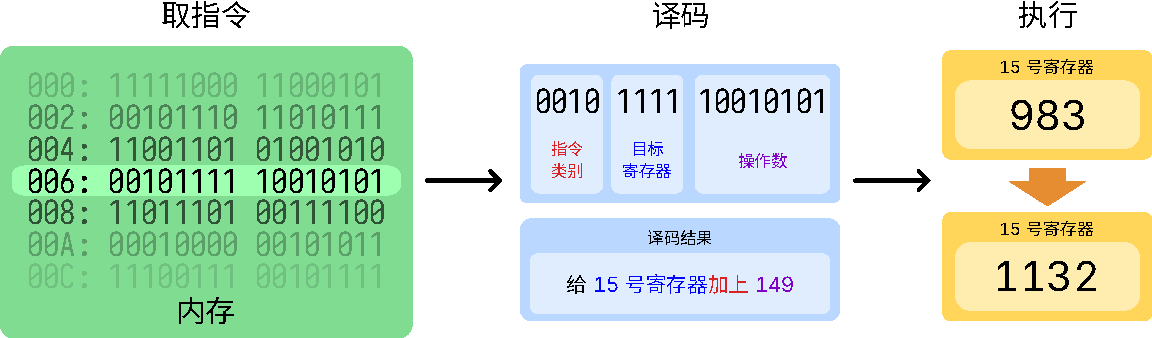
\includegraphics[width=.8\textwidth]{assets/surpass/CPU_exec.pdf}
  \caption{CPU 的工作周期}
  \label{fig:CPU_exec}
\end{figure}

显然,我们的计算机不太能炒菜,它的本职工作是「计算」。因此,计算机的指令世界中,肯定不会有什么「洗菜」「翻炒」这样的指令;相应地,在计算机中,常用指令按照功能可以分成如下几类:

\begin{itemize}
  \item \regcolor{数据传输指令}:它们用来将数据在计算机内部各种地方传递,如从内存中转移到 CPU 内部,或者将 CPU 内部计算好的结果转移到内存。「你缺饭课一号」就有 4 个临时存放食材的碗和一个用来炒菜的锅。在 CPU 内部,也有类似的用来临时存储数据的结构,称为「寄存器」。数据传输指令的主要功能,就是将数据在内存和寄存器中转移。
    \begin{note}
      由于寄存器在 CPU 里面,它的读写速度非常非常快,远远快于内存。不过,现代的处理器中通常只有几个或几十个寄存器,每个寄存器仅能存放几十位的数据,因此对 CPU 来说,寄存器必须珍惜使用,所以才需要频繁传输数据。
    \end{note}
  \item \regcolor{算术与逻辑运算指令}:它们用来执行各种各样的计算,包括算术运算和逻辑运算。算术运算就是诸如「加减乘除」这样的数字运算,而逻辑运算指的是「或、与、非」这些真假条件的判定。
  \item \regcolor{比较与控制流指令}:它们用来实现分支结构和循环结构,主要的功能就是比较、跳转。例如,「无条件跳转」指令在执行后,CPU 就不再会继续执行下一条指令,而是转移到内存中另一处机器代码开始运行;而「大于则跳转」等指令,则会根据两个数的大小关系来决定要不要跳转。
  \item \regcolor{机器控制指令}:它们用来控制整个计算机的运转,包括停机、重置等。
\end{itemize}

随着计算机技术的不断发展,如今,我们常用的电脑 CPU 已经支持上千种不同的指令,上面所展示的只是这个庞大系统的冰山一角。\regcolor{机器代码存放在可执行文件——也就是 \MissingTT{.exe} 文件当中,我们双击运行一个程序,本质就是将它的机器代码装入内存然后执行。}因此,我们在电脑上安装的各种各样的软件,本质就是各种程序的机器代码。

显然,这个将源代码转换为机器代码的过程并不轻松——虽然番茄炒蛋的世界里,一共只有几种操作,但让你手工按照菜谱编写在「你缺饭课一号」上运行的机器代码也不是容易的事;而当这一切面对的是指令上千种、操作类型不计其数的计算机世界时,难度更是堪比登天。好在,早在上个世纪中叶,电子计算机问世之后不久,人们就设计出了自动完成转换过程的程序。借助它,机器能自动地将使用编程语言编写的源代码转换成机器代码。我们把这个过程叫做「\regcolor{编译}」(compile),而这种程序称为「\regcolor{编译器}」(compiler)。\CJKsout*{(所以手动写机器代码的人算不算一种「人形编译器」呢?)}

\begin{note}
  编译器也是一个程序,那它自己是怎么由源代码转换成机器代码的呢?你可以这样理解:第一个编译器是人们用机器代码直接编写的,而当它发展得足够完善之后,人们就可以改用编程语言来设计它,然后由它来编译它自己。这就是编译器的「自举」。
\end{note}

自然,不同的编程语言需要不同的编译器,同一种编程语言也可以有多种不同「品牌」的编译器。例如,C/C++ 最常用的编译器为「GCC」\footnote{GCC(全称「GNU Compiler Collection」,译作「GNU 编译器套装」)包含一系列针对多种语言的编译器,如 C、C++、Objective-C 等)。}「Clang/LLVM」和「微软 Visual C++ 编译器」,它们分别是今天 Linux、macOS 和 Windows 三大操作系统自身主要使用的编译器。Java 则使用「Oracle JDK」或「OpenJDK」提供的编译器——在电脑上玩过游戏《我的世界》(\textit{Minecraft})的读者肯定对这些名字不陌生。

有一些语言,比如 Python,则选择了另外的思路——比起事先将整个程序全部编译成机器代码,这些语言选择在程序运行时逐句完成转换。尽管就结果而言,程序都变成了对应功能的机器代码,但我们把这样的方式叫做「\regcolor{解释}」(interpret),对应的工具则称为「\regcolor{解释器}」(interpreter)。CPython\footnote{之所以叫「CPython」是因为它是用 C 语言写的。这也提醒了我们,一种编程语言的编译器或解释器并不一定要用这种语言自身来编写。} 是 Python 最常用的解释器,也是事实上的官方解释器——如果你在其他地方学习过 Python 编程,你安装的那个可以在 \MissingVerb{>>>} 之后给出单个命令并执行的工具,就是 CPython 解释器。

编译器和解释器填平了从程序到机器的鸿沟:借助它们的力量,我们设计的各种程序终于得以在硬件上运行。不过,世界上的编程语言倒是有成百上千种,那 CPU 所使用的指令难道是一样的吗?或者说,难道世界上所有的计算机,都使用着相同的指令设计吗?答案显然不可能。事实上,在这「不一样」的背后,隐藏着一段像\hyperref[cha:browsers-and-how-to-choose]{\CJKunderwave{浏览器}}那样「明争暗斗」的历史。

\subsection{指令集的明争暗斗}

\subsubsection{从 8086 到 x86-64}

再看看我们的「你缺饭课一号」,这台炒菜机有 4 个临时存放食材的碗,能够接受 8 位长度的指令来执行炒菜动作。我们在之前的指令表格中详细约定了每一种指令的形式和功能。事实上,\regcolor{我们完全可以采用不同的指令格式、不一样的指令长度,甚至也可以选择再增加或者删除一些指令}(比如将「点火」和「倒油」功能分拆成两种指令,或者扩展「点火」指令以控制火候),设计出「你缺饭课二号」「你缺饭课三号」……我们把这样一种\regcolor{对「指令种类、形式、长度等一切相关的东西」的约定,称为「指令集架构」(instruction set architecture,ISA),简称「指令集」}。

我们能自然而然地想象到,在计算机的世界里,指令集肯定也不会是只有一枝独秀的天地,而是百花齐放的花园。但这回,我们的想象与现实之间,有一点点小差距。这个故事还要从 1978 年说起。那一年,美国半导体公司英特尔推出了一款名为「8086」的处理器,看起来如同下图那样,它拥有 8 个寄存器,\regcolor{每个寄存器可以存放 16 位的数据,因此被人们称为「16 位处理器」}。8086 支持约 100 种不同的指令,每种指令长度不一,最短者为 1 字节(8 位),最长者为 6 字节(48 位)。

\begin{note}
  所以,CPU 的「位数」指的就是它的每个寄存器可以存放多少位二进制的数据。
\end{note}

\begin{figure}[htb!]
  \centering
  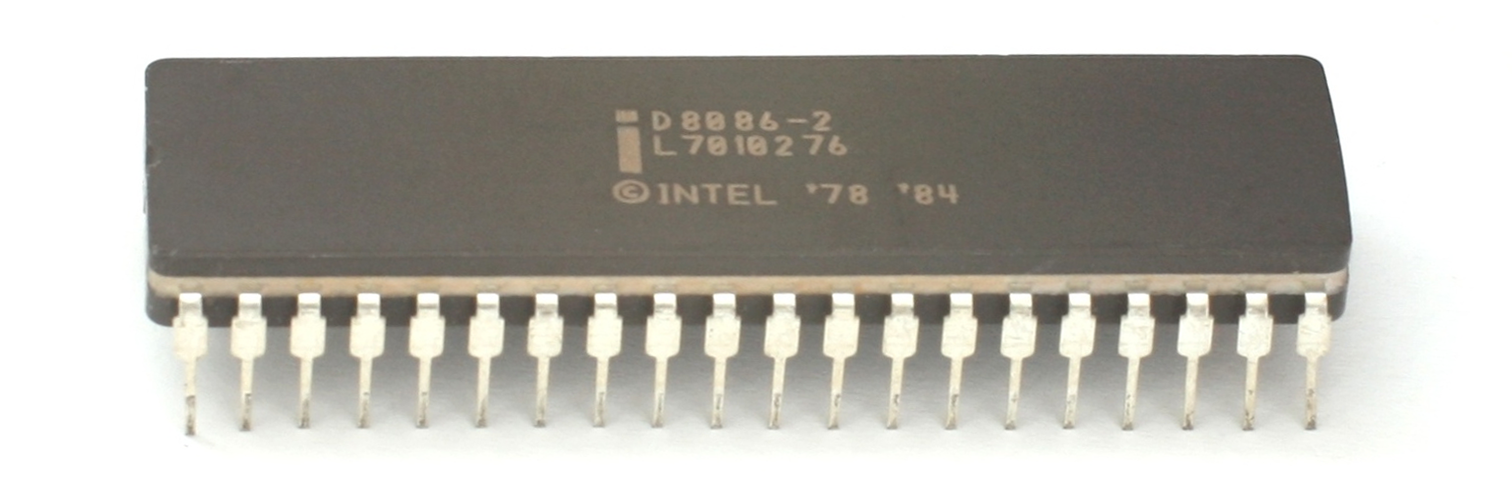
\includegraphics[width=.7\textwidth]{assets/surpass/8086.png}
  \caption{英特尔 8086}
  \label{fig:8086}
\end{figure}

在那个年代,与 8086 同台竞争的 CPU 数量不少,它们大都使用同样的 16 位设计,但是在指令风格、指令数量等方面有差异。按照正常的剧本来说,它应该会和竞品一起在市场上打得「有来有回」,然后一同沉寂在历史的长河中。可是,历史总是充满未知和巧合。当时,IBM 正苦于自己过去几年在个人电脑领域的失败中:IBM 此前拿手的是「大型机」的设计,但传统的设计流程无法适应低端、廉价、小型的个人电脑市场。痛定思痛,IBM 做出了一个大胆的决定:不再拘泥于自己设计 CPU 等硬件,而是把选择交给市场。这时,8086 就入了 IBM 的法眼。

\begin{note}
  「全链条覆盖」和「交给市场」是设计复杂系统的两种思路。历史已经多次告诉我们,这二者间没有固定的「谁好谁坏」的关系,我们必须结合历史条件、产业性质来具体问题具体分析。
\end{note}

1981 年,IBM 发布了名为「IBM PC」的个人电脑,选择 8086 的兄弟型号 8088 作为 CPU。在 8088 处理器的加持下,IBM PC 取得了性能和价格之间不错的平衡,迅速在市场上占据一席之地。同时,IBM 还开放了 IBM PC 的技术参考资料,这意味着其他厂商都可以自由设计、生产和出售与 IBM PC 兼容的软件和硬件,为 IBM PC「外加附件」,甚至能设计出与 IBM PC 本身兼容的电脑。同时,微软也加入了这个\CJKsout{脆弱的}同盟,提供了一套稳定且实用的操作系统 MS-DOS,更是吸引来了许多软件开发商,它们纷纷将自己的软件编译成能在 IBM PC 上运行的机器代码来发布。在这样三重因素的催化之下,\regcolor{IBM PC 很快成为了「个人电脑」的代名词},命运的齿轮从此开始转动。

1982 年,英特尔发布了 8086 的后继产品 80286,它与 8086 使用相同的指令集,但提升了运行的主频,并增强了对内存的访问能力。而到了 1985 年,第三代产品 80386 横空出世。与 8086 和 80286 的显著区别是,\regcolor{80386 将 8 个寄存器的大小升级为了 32 位,标志着它是一颗 32 位处理器}。不过,英特尔并没有选择让它与 8086/80286「割席」,而是通过在它们原本的指令集上额外引入一批指令来支持 32 位相关的功能。这意味着\regcolor{原本能在 8086/80286 上运行的软件可以无需重新编译直接使用},同时以后发布的新软件则可以选择针对 32 位特性引入更强大的功能。这种向后兼容性使得 80386 再一次颠覆市场,再加上便捷易用的 Windows 操作系统横空出世,8086/80286/80386 这三代处理器所使用的指令集逐渐成为了事实上的电脑 CPU 标准。由于这几代产品都使用「80x86」来命名,人们把这套指令集命名为「x86」。

\begin{note}
  在 80386 之后,英特尔把第四代的 CPU 称为「i486」,而第五代的产品则不再使用这种命名,而改为使用「Pentium」(奔腾)这一品牌。歌手朴树在他 1999 年的歌曲 《NEW BOY》中唱道:
  \begin{quoting}
    \centering
    快来吧 奔腾电脑\par
    就让它们代替我来思考
  \end{quoting}

  其中的「奔腾电脑」指的就是使用奔腾 CPU 的电脑。尽管不再以「x86」命名,但是它们的指令集仍然是 x86。
\end{note}

x86 的巨大成功还吸引来了其他一些 CPU 厂商,它们从英特尔那里拿到授权,生产同样使用 x86 指令集,但是自己设计的处理器,这一行列中就包括 AMD。1991 年,AMD 发布了 80386 的复刻版 Am386,随后又发布了 i486 的复刻版 Am486。它们在指令集方面与 80386/i486 完全兼容,凭借更低的价格成为英特尔的有力竞争对手。不过,尽管 AMD 主打价格优势,但是这种总是跟在别人后面模仿的商业路线注定无法成功——芯片技术发展的速度远远快于人们的想像,等复刻品出来,正品早更新换代了。要按照传统剧本,AMD 最终应该会没落于众多 x86 兼容芯片厂商之中,在历史的长河里留下不轻不重的一笔。

然而,转机发生在新世纪来临前的黎明。随着信息技术的飞速发展,人们发现 32 位设计已经有些捉襟见肘:32 位的寄存器只能存放最大为 $2^{32}-1=4\,294\,967\,295$ 的正整数,而当计算任务超过这个数字时,就必须拆分或采用其他的方法,这很大程度上影响了计算效率。同时,受制于同样的原因,32 位架构最大只能使用 4 GB 的内存,尽管在 2000 年前后,4 GB 内存已经是一个巨大的数字,但是当时的人们已经卓有远见地看到了未来。因此,引入更高位数的架构,成为包括英特尔在内的有志之「司」都开始考虑的问题。

我们回看从 80286 到 80386 的 16 位向 32 位的跨越,当时英特尔选择的是在原有指令集的基础上添加新的指令,这样可以在兼容以前的老旧应用时,增加新的功能。然而,在 32 位迈向 64 位这一次,英特尔把步子迈得太大了——他们完全重新设计了一套纯 64 位的指令集(称为 IA-64)。这 IA-64 采用了新的设计思想,支持包括高效的并行计算在内的许多新功能。唯一,但致命的问题是:它与 x86 不兼容,原本的各种软件都需要换用 IA-64 的编译器发布新版本。IA-64 一经面世,世人反应冷淡,这一次英特尔没能成功。

一直以来,我们都经常看见「官方逼死同人」的事情发生,不过这一次,是「同人倒逼官方」。「既然英特尔自己搞 64 位弄砸了,那不正是我 AMD 的好时机吗?」于是,AMD 在 x86 的基础上,直接\regcolor{把原有的 8 个寄存器再扩充成 64 位,再引入一批针对 64 位操作的新指令,不仅实现了 64 位的功能,还在最大程度上保持了对原有 32 位应用的兼容性}。2003 年,AMD 发布 Athlon 64,这是第一块 64 位的 x86 处理器,一经推出,好评不断,随后的两年间,支持 64 位的操作系统和应用软件就开始出现在市场上了。AMD 给这种指令集改了个名,叫「AMD64」。这一次,AMD 的指令集作为「同人作品」,干掉了官方,赢得了胜利。

此时的英特尔有点尴尬——自己推出的 IA-64 无人问津,而身为「同人作者」的 AMD 反而给自己的 x86 升级了。不过,日子还得凑合过嘛……2004 年,英特尔发布了具有里程碑意义的「奔腾 4 Prescott」(Pentium 4 Prescott)处理器。其中一块里程碑,就是使用了 AMD64 指令集,成为了英特尔的第一款 64 位的 x86 处理器。曾经,人们总认为 AMD 的产品是英特尔的仿制品,可是风水轮流转,同人成官方。

当然,英特尔没有使用「AMD64」这个名字。他们把它改名成了「Intel 64」。世人一想,你们这各自拉扯,我们到底应该用哪个名称呢?于是,人们索性\regcolor{用「x86-64」来表示这种 64 位的 x86 指令集},以和原本纯 32 位的 x86 作区分。后来,人们也会\regcolor{把 x86-64 简称为「x64」},用来表示这种指令集。后来的故事,就是我们在第一章\chapref{cha:computer-and-its-components}中所介绍的了那样了——英特尔和 AMD 成为了 x86-64 指令集的两大霸主,开始统治着全世界的电脑 CPU 市场,直到今天。

今天,x86-64 的指令数量已经达到了上千条,是一套名副其实的「复杂指令集」。这其中的一个原因便是 \regcolor{x86 指令集自 8086 诞生以来,就一直采用向后兼容的进化模式}:每一次更新都是在之前的基础上增加功能,因此旧软件基本都能在新硬件上直接使用——即便在今天的最新电脑上,许多近二十年前的软件(比如 Office 2003)仍然能正常运行。这也是 x86 家族指令集能够在桌面电脑领域占据绝对优势的重要原因。

\begin{note}
  得益于这种兼容性,64 位的 CPU 上既可以运行 64 位的操作系统,也可以运行 32 位的操作系统。而在 64 位的操作系统下,也可以同时存在 32 位和 64 位的软件。目前,几乎所有的电脑都在 x86-64 上运行 64 位的操作系统,不过仍然有许多 32 位的软件正在和 64 位的软件共处。打开【任务管理器】,展开【详细信息】并转到【进程】页面,正运行在 32 位的软件后方会用【(32 位)】标出。

  \begin{center}
    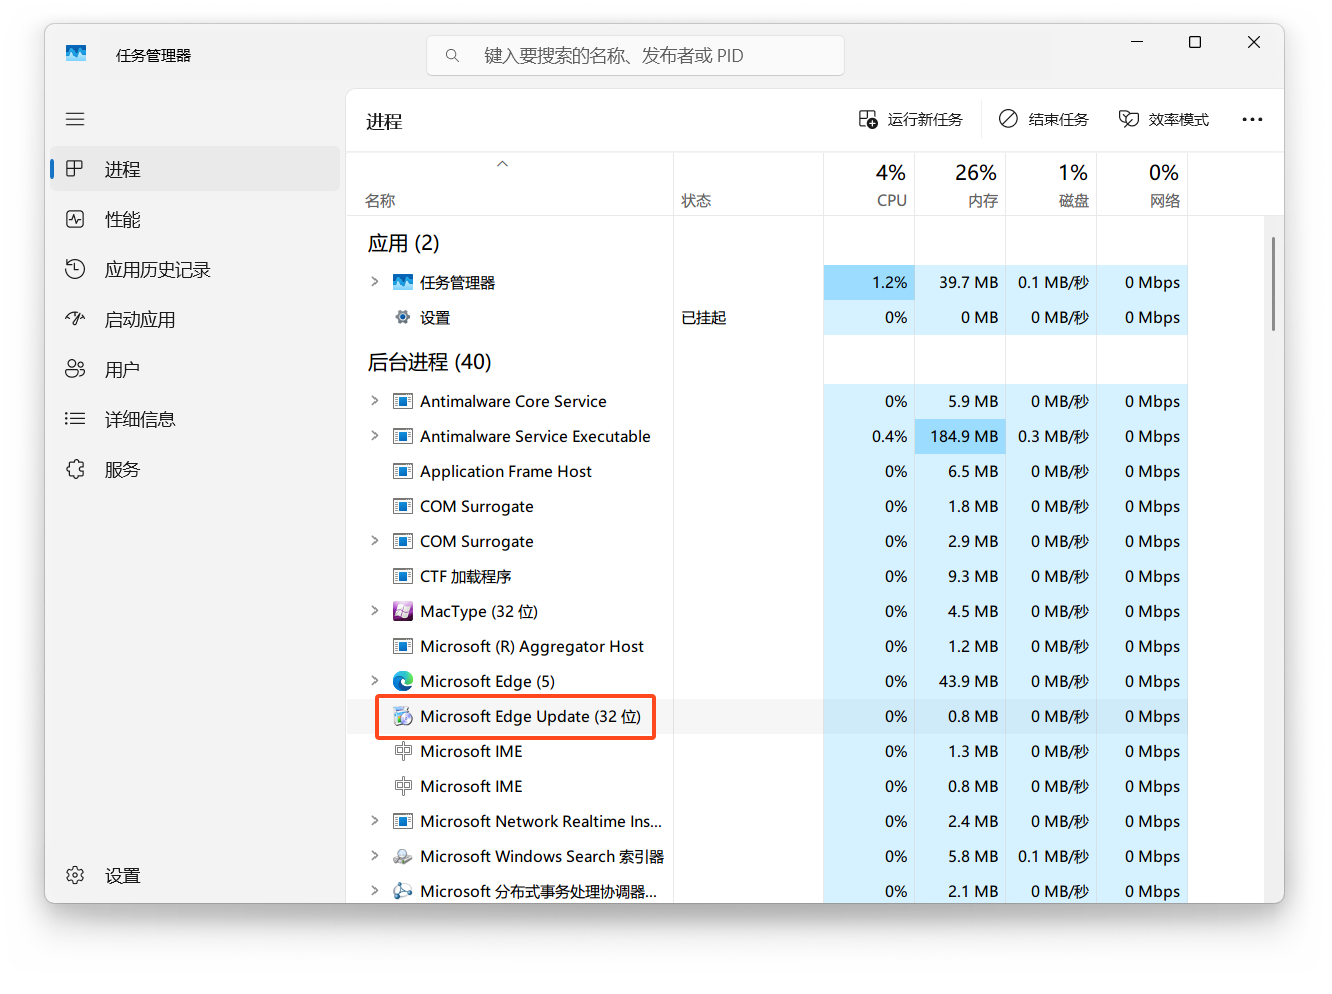
\includegraphics[width=.65\textwidth]{assets/surpass/32bit_in_taskmgr.png}
    \captionof{figure}{任务管理器中的 32 位标记}
    \label{fig:32bit_in_taskmgr}
  \end{center}
\end{note}

对于大多数读者的电脑,右键桌面上的【此电脑】选择【属性】,就能在【设备规格】一栏下方的【系统类型】看见这样一句话:
\begin{quoting}
  64 位操作系统, 基于 x64 的处理器
\end{quoting}
其中「64 位操作系统」说明操作系统本身,以及其上运行的大部分软件都是 64 位的;而「基于 x64 的处理器」,说的就是 x86-64。

\begin{figure}[htb!]
  \centering
  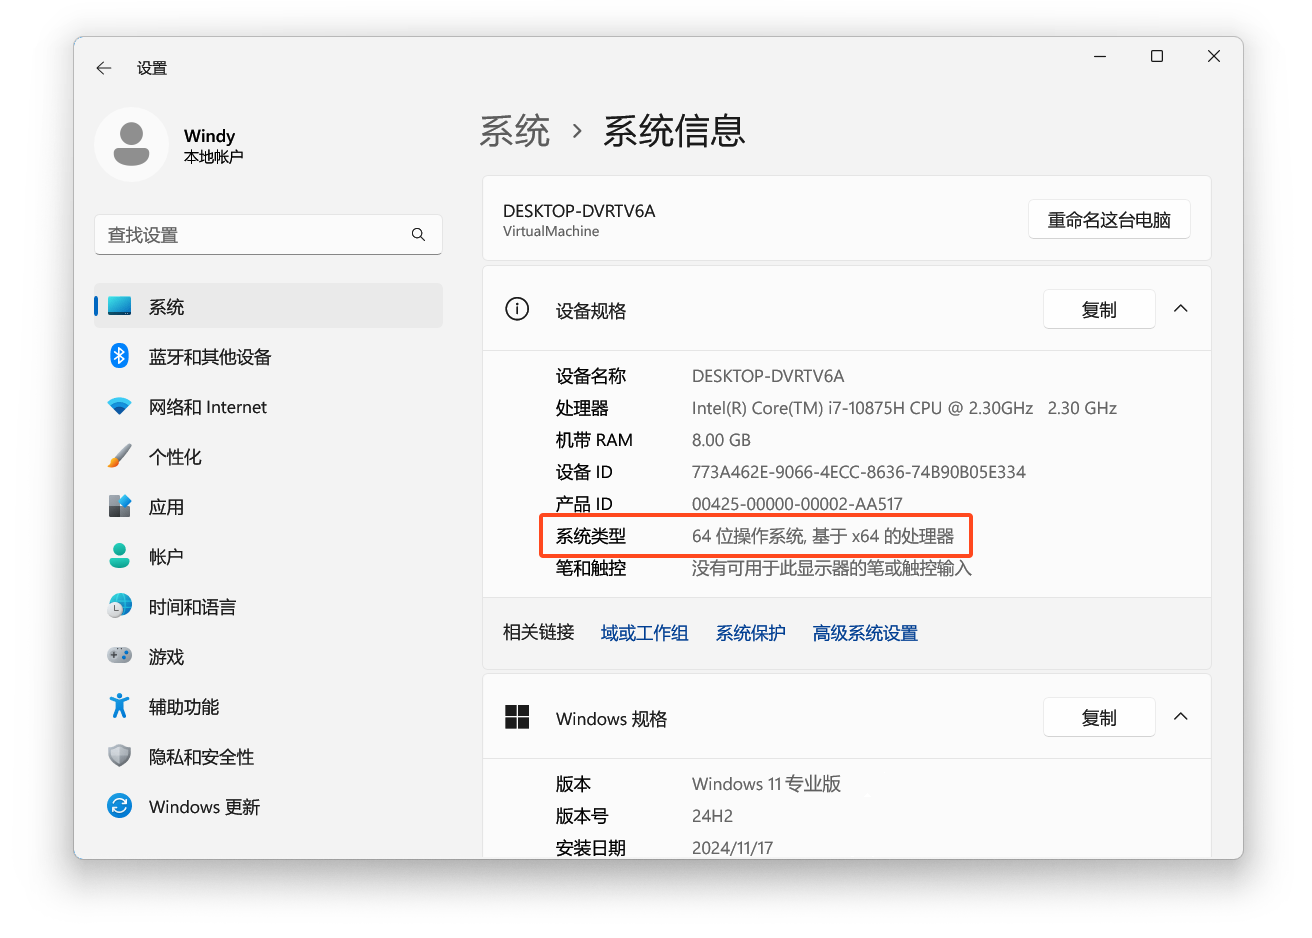
\includegraphics[width=.6\textwidth]{assets/surpass/x64_in_settings.png}
  \caption{系统设置中的指令集说明}
  \label{fig:x64_in_settings}
\end{figure}

\subsubsection{统治移动世界的 ARM}

尽管自 8086 开始,x86 指令集就几乎统治了个人电脑领域。然而,「计算机」不止局限于我们桌子上的个人电脑——无论是手机、平板电脑、MP3 这一众智能设备,还是日用的电视机遥控器、电高压锅、洗衣机等诸多电器,它们的内部也拥有像电脑一样的 CPU 来实现自动控制和人机交互,因而也是一种形式的计算机(称为「嵌入式计算机」)。而在这片属于移动和嵌入式设备的天地中,又是另一派勃勃生机的景象。

1985 年,来自英国的艾康电脑公司(Acorn Computers)发布了一款名叫「ARM1」的原型处理器,「ARM」的含义是「Acorn 精简指令集机器」(Acorn RISC\footnote{是「精简指令集电脑」(Reduced Instruction Set Computer)的缩写。} Machine)。作为一款 32 位处理器,它与同时代包括 80286 在内的 CPU 最大的不同是:\regcolor{它指令集极为简单,只有数十条基本指令},并且舍弃了其他许多处理器中的复杂设计。这种指令集就称为「ARM」指令集。次年,ARM2 投产,\regcolor{精简的设计使得它只需消耗极少的电能,就能实现多样的功能},这为它日后在便捷式设备和微型设备中的大放异彩埋下了伏笔。

\begin{wrapfigure}[7]{r}{7.2cm}
  \centering
  
\includegraphics[width=7cm]{assets/surpass/Arm_logo_2017.pdf}
  \caption{安谋的徽标}
  \label{fig:Arm_logo_2017}
\end{wrapfigure}

时间来到了 90 年代。那时,苹果正计划开发一款可以拿在手上触控操作的「掌上电脑」——可以看成今天 iPad 的前身。低功耗的 ARM 处理器与苹果的产品构思不谋而合。于是,1990 年,苹果、安谋电脑和另一家公司进行了分割重组,直接成立了一家名为「ARM」的公司,中文常译为「安谋」,右边是安谋现在的徽标。「ARM」的名字直接来源于 ARM 系列处理器和 ARM 指令集,不过被重新解释为「高级精简指令集机器」(Advanced RISC Machines)。1993 年,苹果推出了著名的掌上电脑「Apple Newton」(中文常称为「牛顿」),使用的就是 ARM 610 处理器,下图就是一颗 ARM 610 的核心照片。

\begin{figure}[htb!]
  \centering
  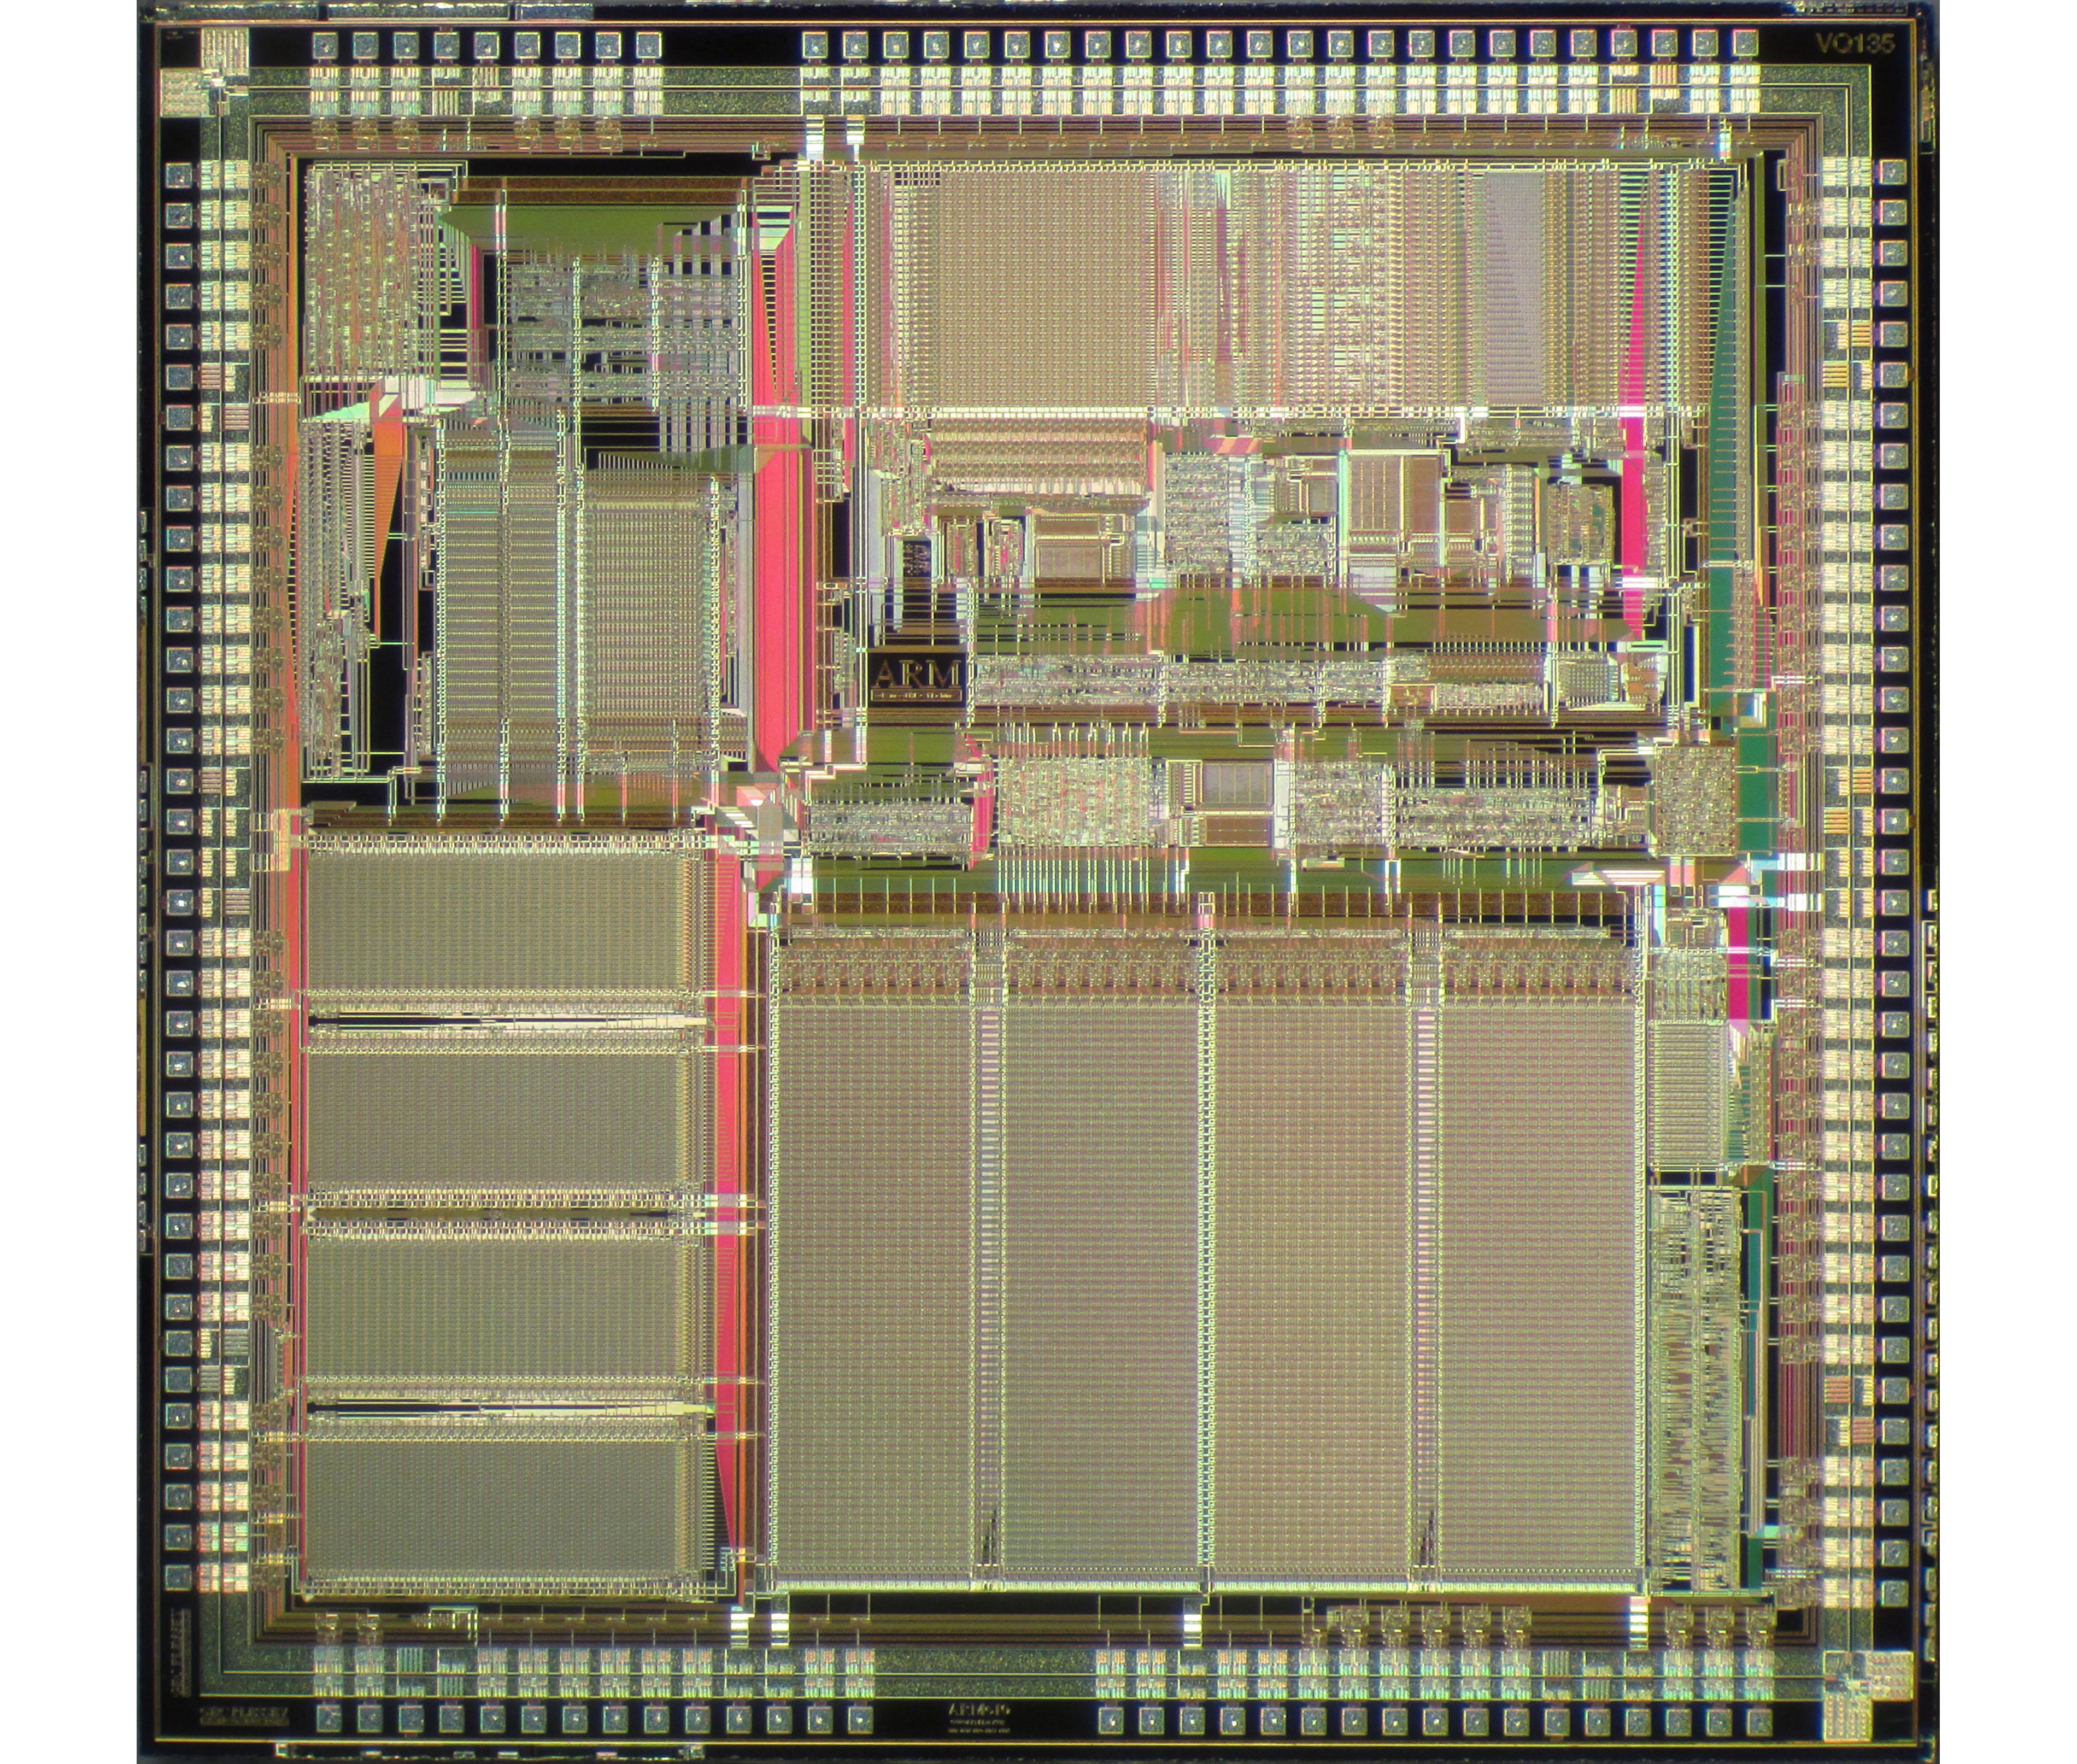
\includegraphics[width=.75\textwidth]{assets/surpass/ARM610_die.jpg}
  \caption{ARM 610}
  \label{fig:ARM610_die}
\end{figure}

在这几年的时间里,尽管 ARM 处理器的性能不断提升,但是其精简的结构设计和低功耗的特点没有改变。安谋敏锐地嗅到了这种低功耗 CPU 市场的商机,开始从造芯片转向卖解决方案——\regcolor{安谋自己不再直接制造和出售 CPU,而是只负责 ARM 指令集的升级、维护,以及在 ARM 指令集上设计出芯片的原型,出售给其他的芯片公司。}其他公司在购得授权后,可以根据原型扩展、组合,并最终设计、制造出自己品牌的,但采用 ARM 指令集的 CPU。站在后来者的视角,我们不得不感叹这种模式的强大之处:越来越多的企业借 ARM 指令集入局市场,带来良性竞争和发展,而安谋则依靠授权费用不断发展,继续让 ARM 指令集变得更加强大。

进入 21 世纪以来,移动设备和嵌入式系统迎来崛起。如果说 x86(以及 x86-64)是事实上的个人电脑指令集标准,那么 ARM 无疑则是事实上的移动设备指令集标准。一方面,高通、三星、联发科、德州仪器等老牌芯片厂商入局 ARM,让 ARM 指令集的 CPU 选择越来越多;另一方面,智能手机、平板电脑等便携式电子设备的快速发展,又反过来促进了相关芯片产业前行。

今天,ARM 指令集的 CPU 在我们身边无处不在。无论是 iPhone 使用的苹果 A 系列 CPU,还是各品牌安卓手机所使用的「高通骁龙」「联发科天玑」等系列 CPU,又或是华为手机使用的「海思麒麟」CPU,它们都使用的是 ARM 指令集。而在许多小型智能设备,如门禁机、打卡机、扫地机器人中使用的「STM32」系列芯片,也使用的是 ARM 指令集。说 ARM 指令集「统治」了移动世界,一点都不为过。

\begin{note}
  ARM 指令集是一个非常灵活的指令集,面向不同的应用场景,它有许多不同的版本,其中可以选配各种功能。例如,用在打卡机上的 ARM 指令集,要比用在智能手机上的要简单得多。
\end{note}

看到这儿,我们自然而然会想到一个问题:现在,手机和平板电脑的性能已经非常强大,玩游戏、剪视频,甚至轻度的工作都可以胜任,这证明 ARM 能在低功耗的同时具有非常高的上限,用武之地也不会只局限在移动设备上。反观 x86-64,厚重的历史包袱似乎让它有点儿喘不过气。那为什么在个人电脑领域,仍然是 x86-64 的天下呢?解决这个问题的答案,又要回到软件头上。在下一节「应用生态」,我们将揭晓答案。

\subsubsection{用开放拥抱自主}

无论是 x86-64 还是 ARM,它们都有一个特点:受商业公司控制。虽说除了英特尔和 AMD 之外,仍然有数家企业取得了一部分 x86-64 的授权,但是它们的市场份额几乎可以忽略不计,而当下英特尔和 AMD 这俩巨头肯定也不会舍得将蛋糕再分给他人。而在 ARM 这边,想要获得 ARM 指令集的授权,也需要向安谋支付高昂的授权费用。在软件的世界里,我们有自由和开源软件这样开放共享的存在,那在指令集的世界中,是否存在类似的想法呢?答案是肯定的。

2010 年,加州大学伯克利分校提出了一套名为「RISC-V」指令集。\regcolor{这是一套开源指令集,在一定的条件下,它可以自由地用于任何目的,允许任何人设计、制造和销售使用该指令集的芯片,而不必支付任何费用。}RISC-V 指令集在公开之后,获得了来自许多高校、企业和研究机构的关注——毕竟,和自由软件的「众人拾材火焰高」一样,共同建设 RISC-V 指令集,最终亦能使自己受益。十多年来,RISC-V 的关注度一路高涨,并且也已经有了商业的和开源的芯片实现,如阿里旗下的达摩院推出的玄铁 910 CPU,以及中科院的「香山」CPU。尽管目前对 RISC-V 的实际应用仍然处于实验室阶段,但它的表现已经未来可期。

除了 RISC-V 之外,我国芯片公司龙芯也在 2021 年发布了一套全新的指令集「LoongArch」,中文称「龙架构」,并稳步推出了几代 CPU 产品,均具有极为出色的性能表现,下图是龙芯官网对 3A6000 CPU 的介绍。龙架构除了基础部分开源外,还有一个至关重要的特点——自主。这一特点在今天的变局之下显得极为重要:以 ARM 指令集为例,尽管理论上只要购买授权就能设计出自己的 ARM 指令集处理器,但是「卖不卖给你」这事儿,也得由人家说了算。2019 年,中美贸易摩擦正激烈的时候,网上就有人开始讨论 ARM 是否会停止对华为的授权。尽管目前华为拥有 ARMv9 的永久授权,但当下的国际形势风云变幻,谁也无法预料「脱钩」是否真的会发生。而对于自主可控的指令集,就不存在这样的风险。这不断警醒我们:自主,极为重要。

\begin{figure}[htb!]
  \centering
  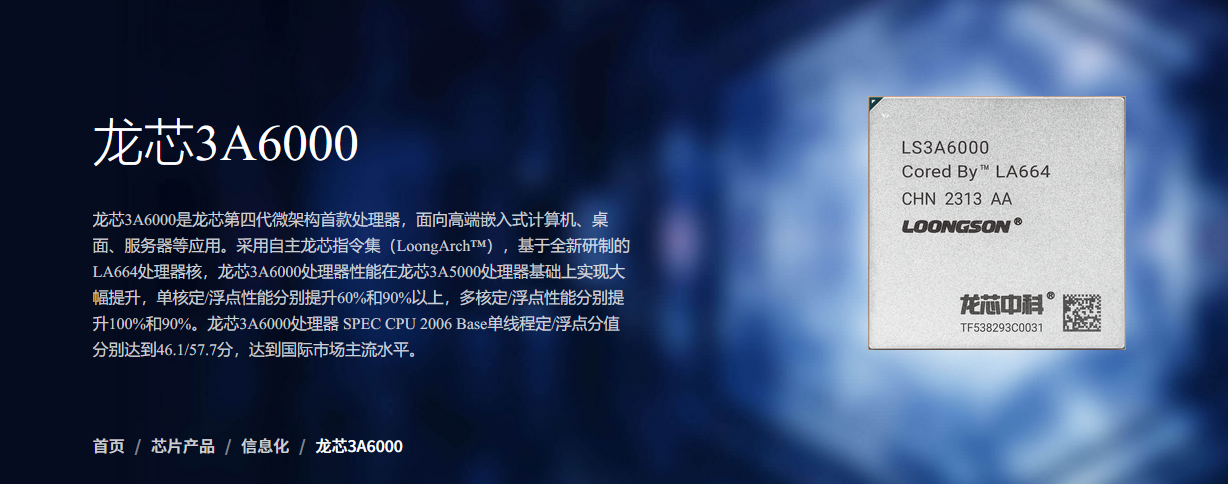
\includegraphics[width=.8\textwidth]{assets/surpass/LS3A6K_webpage.png}
  \caption{龙芯官网的 3A6000}
  \label{fig:LS3A6K_webpage}
\end{figure}

就像龙架构的诞生一样,开放和自主并不矛盾;相反,它们在很多时候,是一体两面的统一。用开放拥抱自主,是当下处于变局之中的我们最好的选择。

\subsection{应用生态与转译}

在介绍 ARM 指令集时,我们留下了一个疑问:明明 ARM 指令集的上限很高,功耗又更低,没有那些「历史包袱」,可为什么今天在个人电脑领域,ARM 远无法与 x86-64 平分秋色?进一步说,RISC-V、龙架构这些新兴指令集,为什么难以在市场上推进?一切的根源便是由软件构造起来的「应用生态」。

显然,\regcolor{为一种指令集编译的软件,无法直接在另一种指令集的处理器上运行}。例如,在 ARM 指令集的 CPU 上,无法直接运行 x86-64 的机器代码。这使得使用不同指令集的 CPU 之间形成了一层层厚障壁,软件无法直接穿过。\regcolor{我们把为某个指令集编译的所有软件组成的整体,称为这个指令集的「应用生态」。}

不难想到,由于 x86 指令集在历史上的成功,在 x86 和 x86-64 指令集上,已经构建起了巨大无比的应用生态。从 Windows 操作系统本身开始,我们所使用的几乎一切电脑软件,都提供了为 x86 或 x86-64 指令集编译的机器代码。我们能够在网上直接下载一款 app 并双击运行,就是因为厂商已经默认所有人都在使用这套指令集的 CPU。如果我们需要改用 ARM 指令集的 CPU,\regcolor{最根本的办法,就是要求所有软件厂商,使用针对 ARM 的编译器,重新编译它们的软件}。这显然有一定的难度。

如果存在比较封闭的软件生态(即常用软件的数量不多、且软件厂商可控),只要有足够的时间,这么做并非完全不可行。2020 年,苹果发布了采用 ARM 指令集的电脑处理器 M1,并推出了搭载该芯片的电脑——此前,苹果的电脑产品亦使用英特尔的处理器。由于本身在 macOS 上的软件支持就相对较少,同时苹果又有极强的行业号召力,到了 2024 年,ARM 指令集的的苹果电脑已经有了相当数量的软件支持。又得益于 ARM 指令集较为高效的设计,这些电脑产品在日常办公、平面设计乃至软件开发等少数专业领域也有了不错的体验。

但这样的成功难以在 Windows 平台上复刻——面向 Windows 平台的软件多如牛毛,即使微软再有能力,也难以逐个联系它们的开发者,要求使用针对 ARM 的编译器重新编译软件。既然让软件厂商在一夜之间全部完成转变不太现实,人们想出了另一种折中的方案:能不能设计一种「现场翻译器」,一句一句将某指令集的指令「翻译」为另一指令集的指令呢?这就是「转译」,如下图所示。

\begin{figure}[htb!]
  \centering
  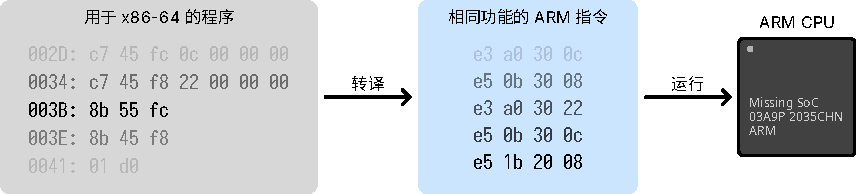
\includegraphics[width=.85\textwidth]{assets/surpass/Translate.pdf}
  \caption{转译}
  \label{fig:Translate}
\end{figure}

实际上,苹果在推出使用 ARM 指令集电脑的同时,亦发布了一款称为「Rosetta 2」\footnote{为什么有「2」呢?其实苹果电脑在本世纪初还经历过一次指令集转换:从一种名为「PowerPC」的指令集迁移到 x86-64。当时苹果也推出了一款转译器,称为「Rosetta」。顺带一提,Rosetta 一名来源于古埃及的罗塞塔石碑,其上刻有同一段内容的三种不同语言版本。它的出土让考古学家得以解读已经失传千年的古埃及象形文字。}的转译器,对于那些过去编译的、针对 x86-64 指令集的应用,macOS 使用该转译器来在 ARM 指令集的处理器上运行。这为软件厂商的转变腾出了宝贵的窗口期。然而,转译最大的问题便是性能:可以想象,原本一条指令就能执行的事,由于转译本身存在的开销,就要用许多条指令才能完成了。同时,转译并不是完美的——如果一些软件的设计本身就依赖 x86-64 指令集的独有特性,那转译也无能为力。

如果说苹果借助自己的影响力和 Rosetta 2 转译器,勉强实现了从 x86-64 到 ARM 的过渡,那这个问题在 Windows 身上,就不那么顺利了。尽管 Windows 自身早已推出了支持 ARM 指令集的版本,但是在应用软件方面,Windows 要比 macOS 更加依赖转译——可是,转译带来的问题客观存在,这就注定了 Windows 上的 ARM 指令集生态更难构建。虽然市面上如今已经可以见到少量采用 ARM 指令集 CPU 的 Windows 电脑\footnote{这些电脑通常使用高通的处理器。},但它们的使用体验仍然有比较大的进步空间。

\section{编程:从工具到桥梁}

现在,相信对「程序是什么」「编程在做什么」以及「程序如何在电脑硬件上运行」三个问题,你在心中已经有了答案。今天,各种各样的「编程培训」广告无处不在,从小学生到职场人士,似乎都在学习编程。最初,编程只是计算机与人类沟通的工具,但时过境迁,它逐渐成为了连接人与机器的桥梁。跨越「编程之桥」,我们将抽象的思想创生为现实的无尽力量,将复杂的挑战转化为优雅的解决方案。

\subsection{「编程对我能有什么用?」}

编程最直观的价值在于,我们能用自己的思路解决实际问题,它让普通人不再局限于使用工具,而更能自己去创造工具。面对工作、学习或生活中的各种需求,我们可以通过编程,为这些需求量身定制解决方案。相信你在生活和学习中,一定遇到过「现有的软件好像没有提供我要的功能」的情况——比如,\regcolor{根据一个 Excel 电子表格中的名单,给每个人单独新建一个文件夹}。无论是 Windows 系统本身还是 Excel 软件,都不存在一键完成它的功能。但这也无可厚非:这个需求并不普遍,软件厂商几乎不会因为少数人的要求去增加功能。

\begin{figure}[htb!]
  \centering
  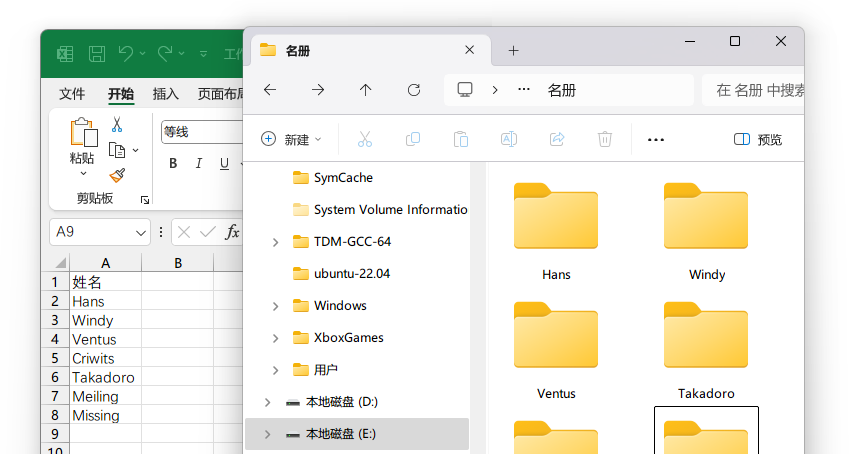
\includegraphics[width=.65\textwidth]{assets/surpass/Sheet_and_folders.png}
  \caption{名册和文件夹}
  \label{fig:Sheet_and_folders}
\end{figure}

但这种需求显然在办公和学习场景中存在,难道我们就只能手工逐个新建吗?实际上,只要自己编写一个不到十行代码的简单程序,我们就可以将这个过程自动化。以 Python 语言为例,下面的代码就能完成这个任务。

\begin{MissingVerbatim}[python]
  import pandas as pd
  import os

  # 读取 Excel 文件
  df = pd.read_excel("path_to_your_excel_file.xlsx")

  # 获取姓名列
  names = df["姓名"]

  # 创建文件夹
  for name in names:
      os.makedirs(name, exist_ok=True)
\end{MissingVerbatim}

即使需求变得复杂,比如「给文件夹加上编号」「区分性别」「按部门新建」,甚至「新建文件夹后,将对应人员的照片按规则命名后放入」等等,都只需要简单修改代码就能解决。通过编写程序,我们给自己创造了适应具体任务的「工具」,减轻了自己的工作量。往大了说,编程是开启电脑潜力的钥匙,让我们不再局限于既有的功能,而是能主动探索与创新。

当然,学习编程还有一些老生常谈的优势,例如培养逻辑思维和抽象能力:编程的过程要求我们把一个复杂的问题拆解为清晰的步骤,并以精确的语言描述解决方法。这种思维模式能显著提高我们分析问题、组织思路的能力,让我们遇到问题时优先去思考「如何解决」而不是怨天尤人。正因为如此,编程已经被看作一种类似阅读、写作和数学的基础技能,能够拓展我们的思维方式。

但或许有人会说:「我学了编程,可我并不觉得它有什么用。而且我也没怎么用到它。」作为一门技能,编程遵循「用进废退」的模式。如果你遇到问题时,不去想怎么使用新获得的技能去解决问题,那么这门技能永远会处在衰退的路上。反之,如果你尝试使用编程思维去思考问题,那么编程技能会得到正反馈,你会习惯于这种思考模式,久而久之,分析解决复杂问题如同抽丝剥茧——虽不容易,但总会成功。

这就是学习编程的真谛:\regcolor{去培养逻辑思维、去学会拆解问题、去提高解决问题的能力、去创造独属自己的工具。}因此,无论是为了解决实际问题,还是为了培养更好的思维方式,或是想让生活更加容易,抑或是为了更高效地使用电脑,编程都能为我们提供重要的助力。

今天,这股已经吹到大江南北的「学习编程」之风,已经吹进了中小学,以各色各样「程序竞赛」的形式出现。然而,当各种程序竞赛成为家长和学生的「心头肉」时,我们就需要谨慎行事了。

\subsection{毋揠苗助长,宜脚踏实地}

编程作为一项技能得到普及,是社会进步的必然趋势。然而,中小学的编程教育,不能说是蔚然成风,却更像是追名逐利:各种竞赛与加分的说辞甚嚣尘上,\regcolor{学习编程的初衷,逐渐被竞赛和升学压力所裹挟}。虽然一些家长明白编程思维的益处,却为了「不输在起跑线上」,希望孩子尽早接触编程。这实际上是急功近利的行为——低龄的孩子,基础数理知识「一穷二白」,计算机操作都成问题,何德何能学习编程?但为了奖状和证书,他们不得不疲于奔命。如此揠苗助长,不仅不能培养编程思维,更违背了客观规律,最终令孩子反感计算机与「程序」的任何有关话题。

事实上,相信许多人对计算机的兴趣,都是从一些网站上的小游戏开始的。当年的我们,不知道游戏中的按钮上写的是什么,但亲自尝试之后,知道了「点【PLAY】可以玩」「点【OPTION】是设置」「点【QUIT】是退出」……这种探索未知的快乐,深深印刻在了我们幼小的心灵中,并保留到了现在。人常说:「兴趣是最好的老师。」幼时依靠天性培养的兴趣,会令心中的种子破土发芽,加以引导与呵护,有朝一日终能长成参天大树。

再看初等和中等教育阶段。按理说拥有了一定基础,这一阶段,培养编程思维将会更容易。然而,一些学校的编程学习,只是死背概念、硬做题;又有一些学校只将眼光放在奥赛,却不普及计算机基础知识。学习编程的真谛被功利化的教育模式冲淡,培养出来的学生却不知计算机的基本知识,这是病态而不科学的。我们时不时看到如此割裂的现实:许多中小学在程序设计竞赛上屡传捷报,但是更多的人却以「电脑小白」的身份步入社会\footnote{比如 \url{https://www.bilibili.com/video/BV11w4m1y7kA/} 这样的},甚至给了《你缺计课》这样的作品诞生的空间。

种种现象,都要归结到一个问题——「编程教育为了什么?」回顾我们上一节点出的「编程之真谛」,这个问题的答案呼之欲出:编程教育的价值,在于为我们——每一位生活在信息时代的人——提供一个帮手,一件能创造工具、提升效率的有力工具。不是每个人都是程序员,也不是每个人都要靠编程赚钱,对大多数人而言,它是一门技能、一种素养。但在得到这种素养之前,学习计算机基础知识显然尤为必要。这就是《你缺失的那门计算机课》的初衷与使命。我们不教编程,但教「何为编程」;我们不教使用软件,但我们教「如何学习使用软件」;我们不教装配、制造计算机,但我们教「计算机各部分的作用」……我们希望能做到脚踏实地,也希望计算机基础教育同样如此。

\subsection{用创造、创新与思考开启未来}

在已经进入「万物互联」时代的今天,计算机与程序的重要性正日益凸显。虽然我们说了许多「学习编程不宜过早、揠苗助长」的话,但另一面却不是如此——尝试编程思维,无论何时都不晚。

程序语言与计算技术是计算机得以运作的基础,而学习编程,不仅仅是掌握一门技能,更是在与这信息时代对话。从头脑中的思维之弦奏出的韵律,到计算机中 0 与 1 完成的圆舞曲,我们与它们共谱数字的乐章,将一个个问题拆解、消弭。这正是信息时代得以建立的基石,也是我们超越这个时代所必需的能力。

在这个时代,计算机随处可见,它们已经构成了我们生活的一部分。在这代码驱动的世界中,编程让我们有机会成为参与者,而不仅仅是旁观者。从人工智能到虚拟现实,从金融科技到社会公益,编程为我们打开了无数可能性的大门。我们应当思考,思考如何借助程序解决人们面临的挑战;我们需要创新,创新使用程序的语言去应对纷繁复杂的问题;我们可以创造,创造一个人与万物共同进步的美好未来。

也许,下一个改变世界的程序,就来自于此刻阅读本书、探索未知的你。

\practice

\begin{enumerate}
  \item 尝试把学习生活中的某项任务用「大事化小」的程序思维描述一遍;
  \item 上网搜索,了解文中提到的一些编程语言,不必真的去学(不过学一门也不是不行);
  \item 尝试用自己的话说说从编程语言,到程序的机器代码,再到机器运行程序,一路上发生了什么;
  \item 查找一下你常用的软件有没有适用于不同指令集体系的版本。
\end{enumerate}